\section{Annexe calibration photométrique}
\begin{figure}[h]
        \centering
        \includegraphics[width=0.6\linewidth]{fig/annexe flux.pdf}
        \caption{Flux corrigé du fond de ciel en fonction du rayon d'ouverture pour différentes étoiles}
        \label{annexe flux}
\end{figure}
\hfill
\begin{figure}[h]
        \centering
        \includegraphics[width=0.55\linewidth]{fig/snr1.pdf}
        \caption{Rayon optimal déterminé par la méthode du critère RSB sur l'étoile avec le plus faible pic}
        \label{gannexe RSB1}
\end{figure}

 \begin{figure}[h]
     \centering
     \begin{subfigure}[b]{0.33\textwidth}
         \centering
         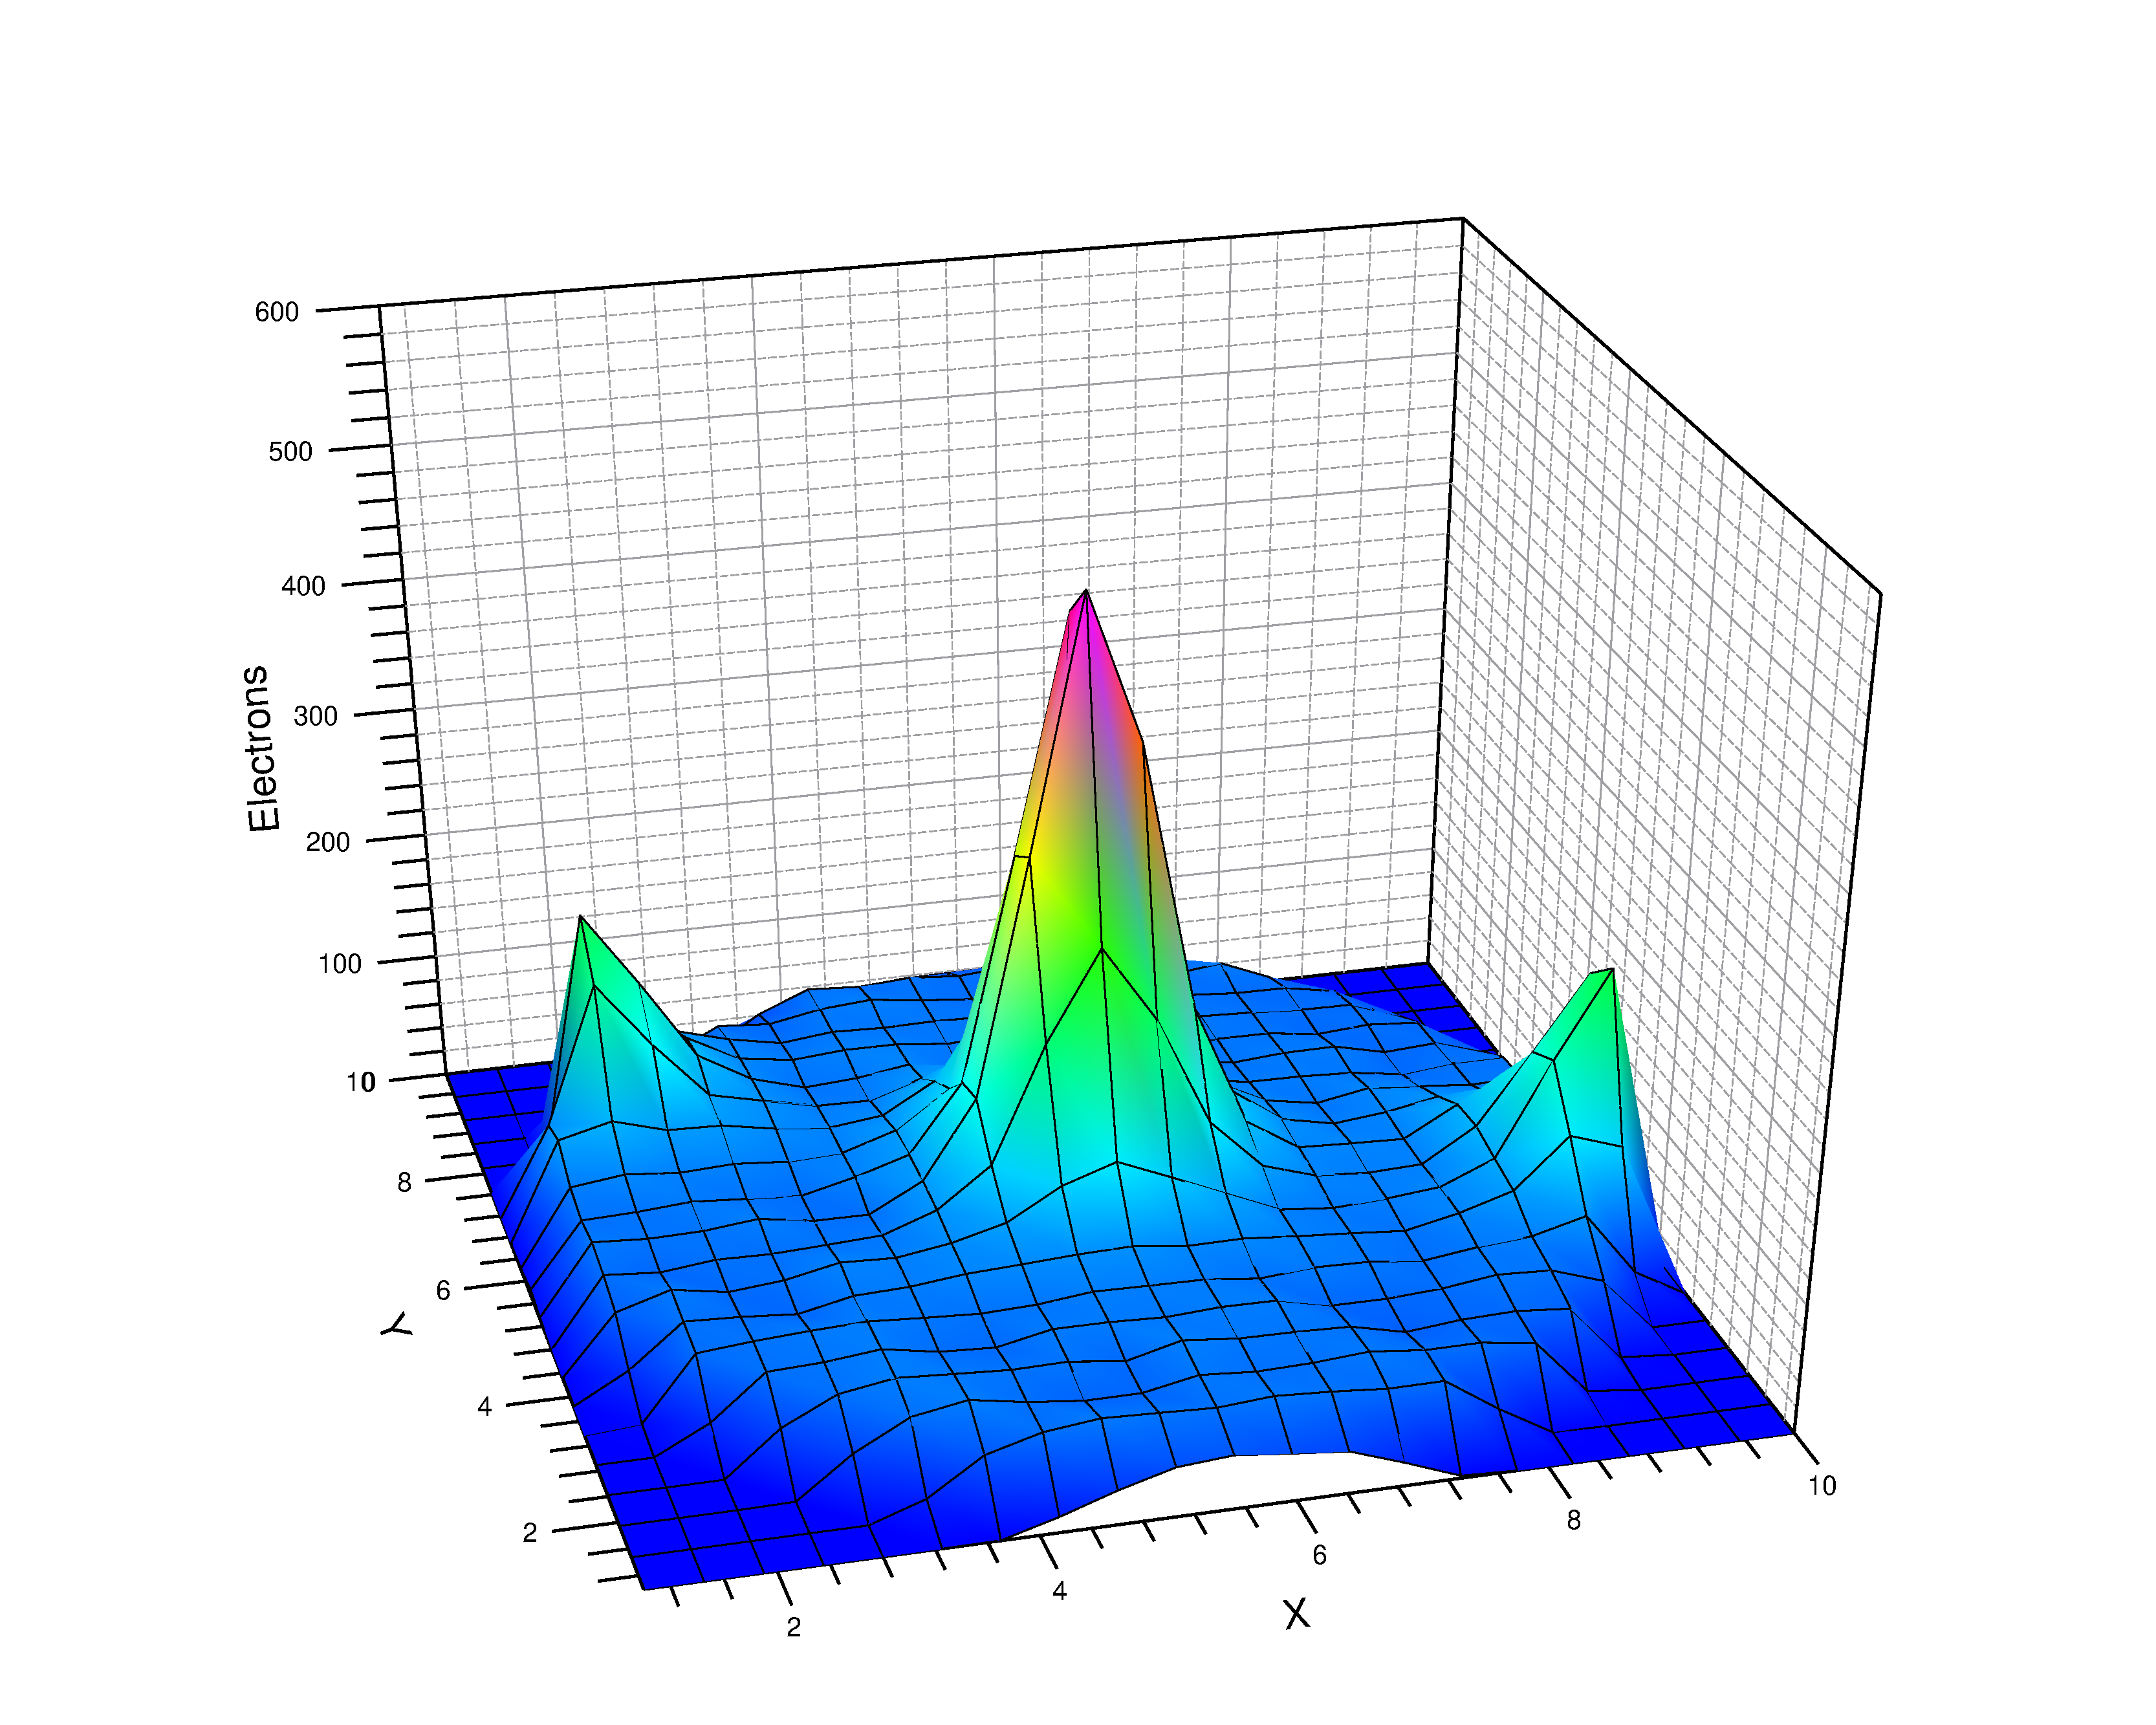
\includegraphics[width=1\textwidth]{fig/etoile divergente red1.pdf}
         \caption{Première étoile exclue}
         \label{subfig:excl1}
     \end{subfigure}
     \hfill
          \begin{subfigure}[b]{0.33\textwidth}
              \centering
              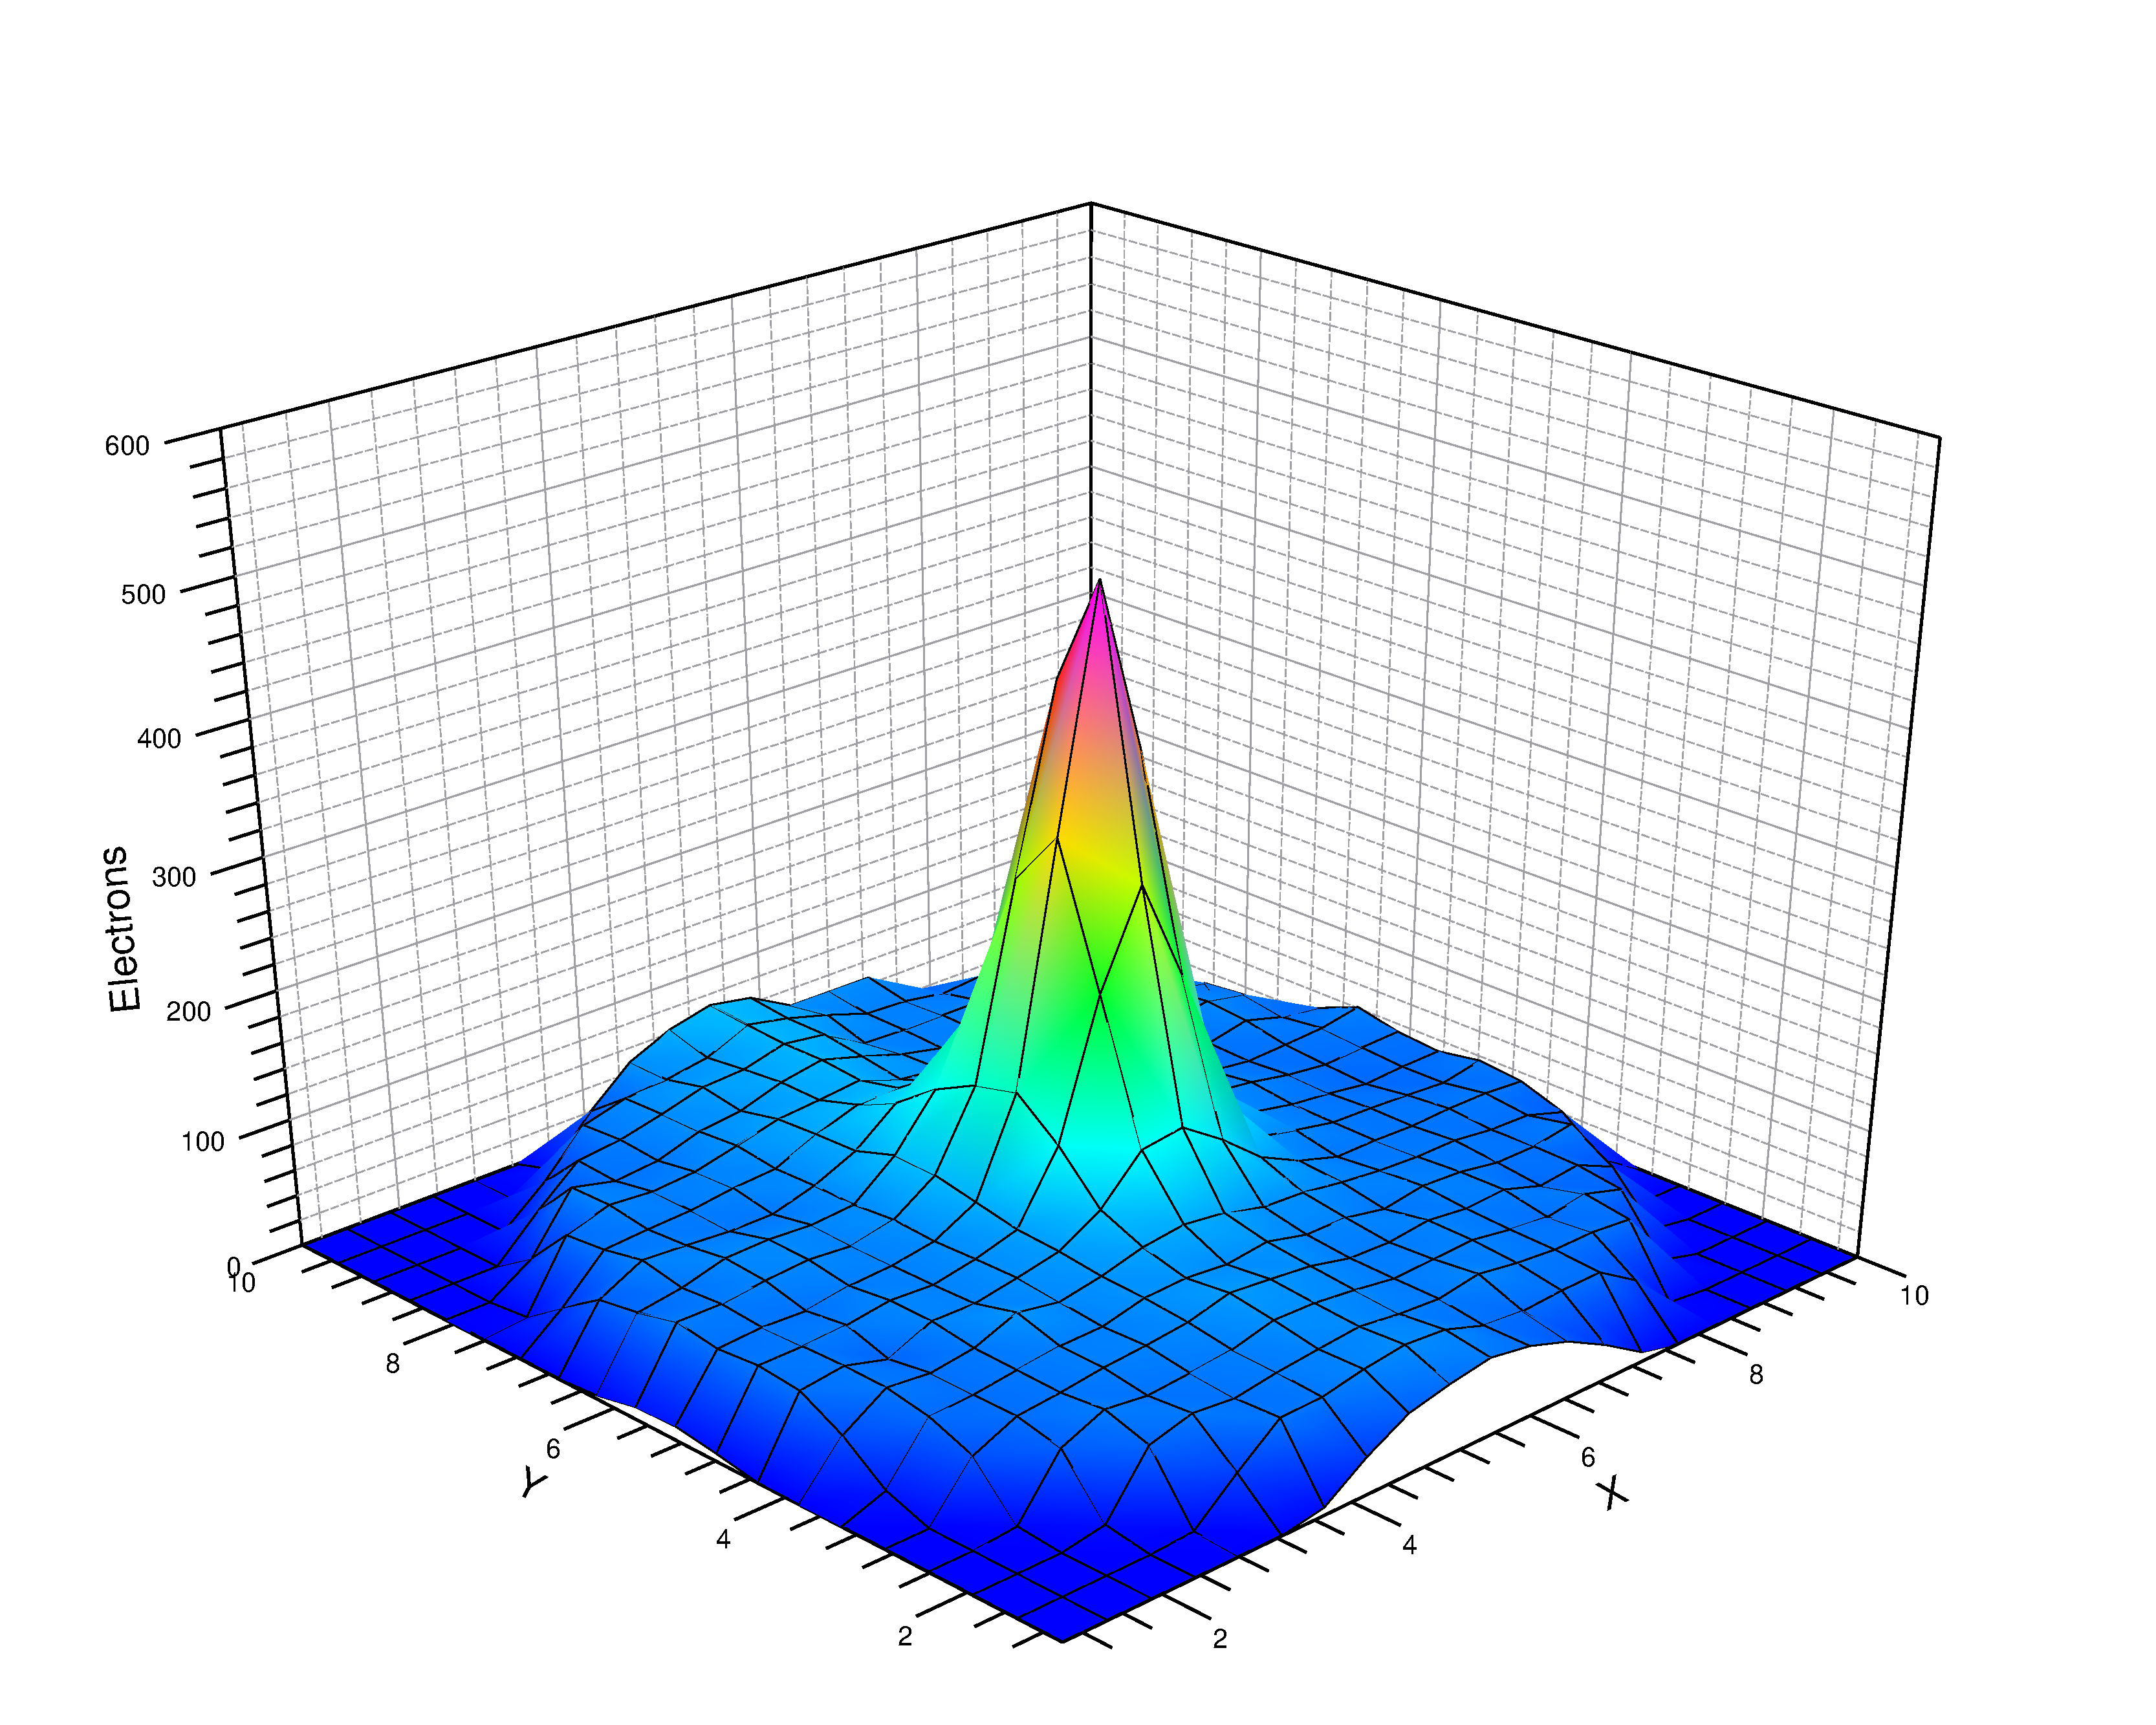
\includegraphics[width=1\textwidth]{fig/etoile divergente red2.pdf}
              \caption{Seconde étoile exclue}
              \label{subfig:excl2}
          \end{subfigure}
      \hfill
           \begin{subfigure}[b]{0.33\textwidth}
               \centering
               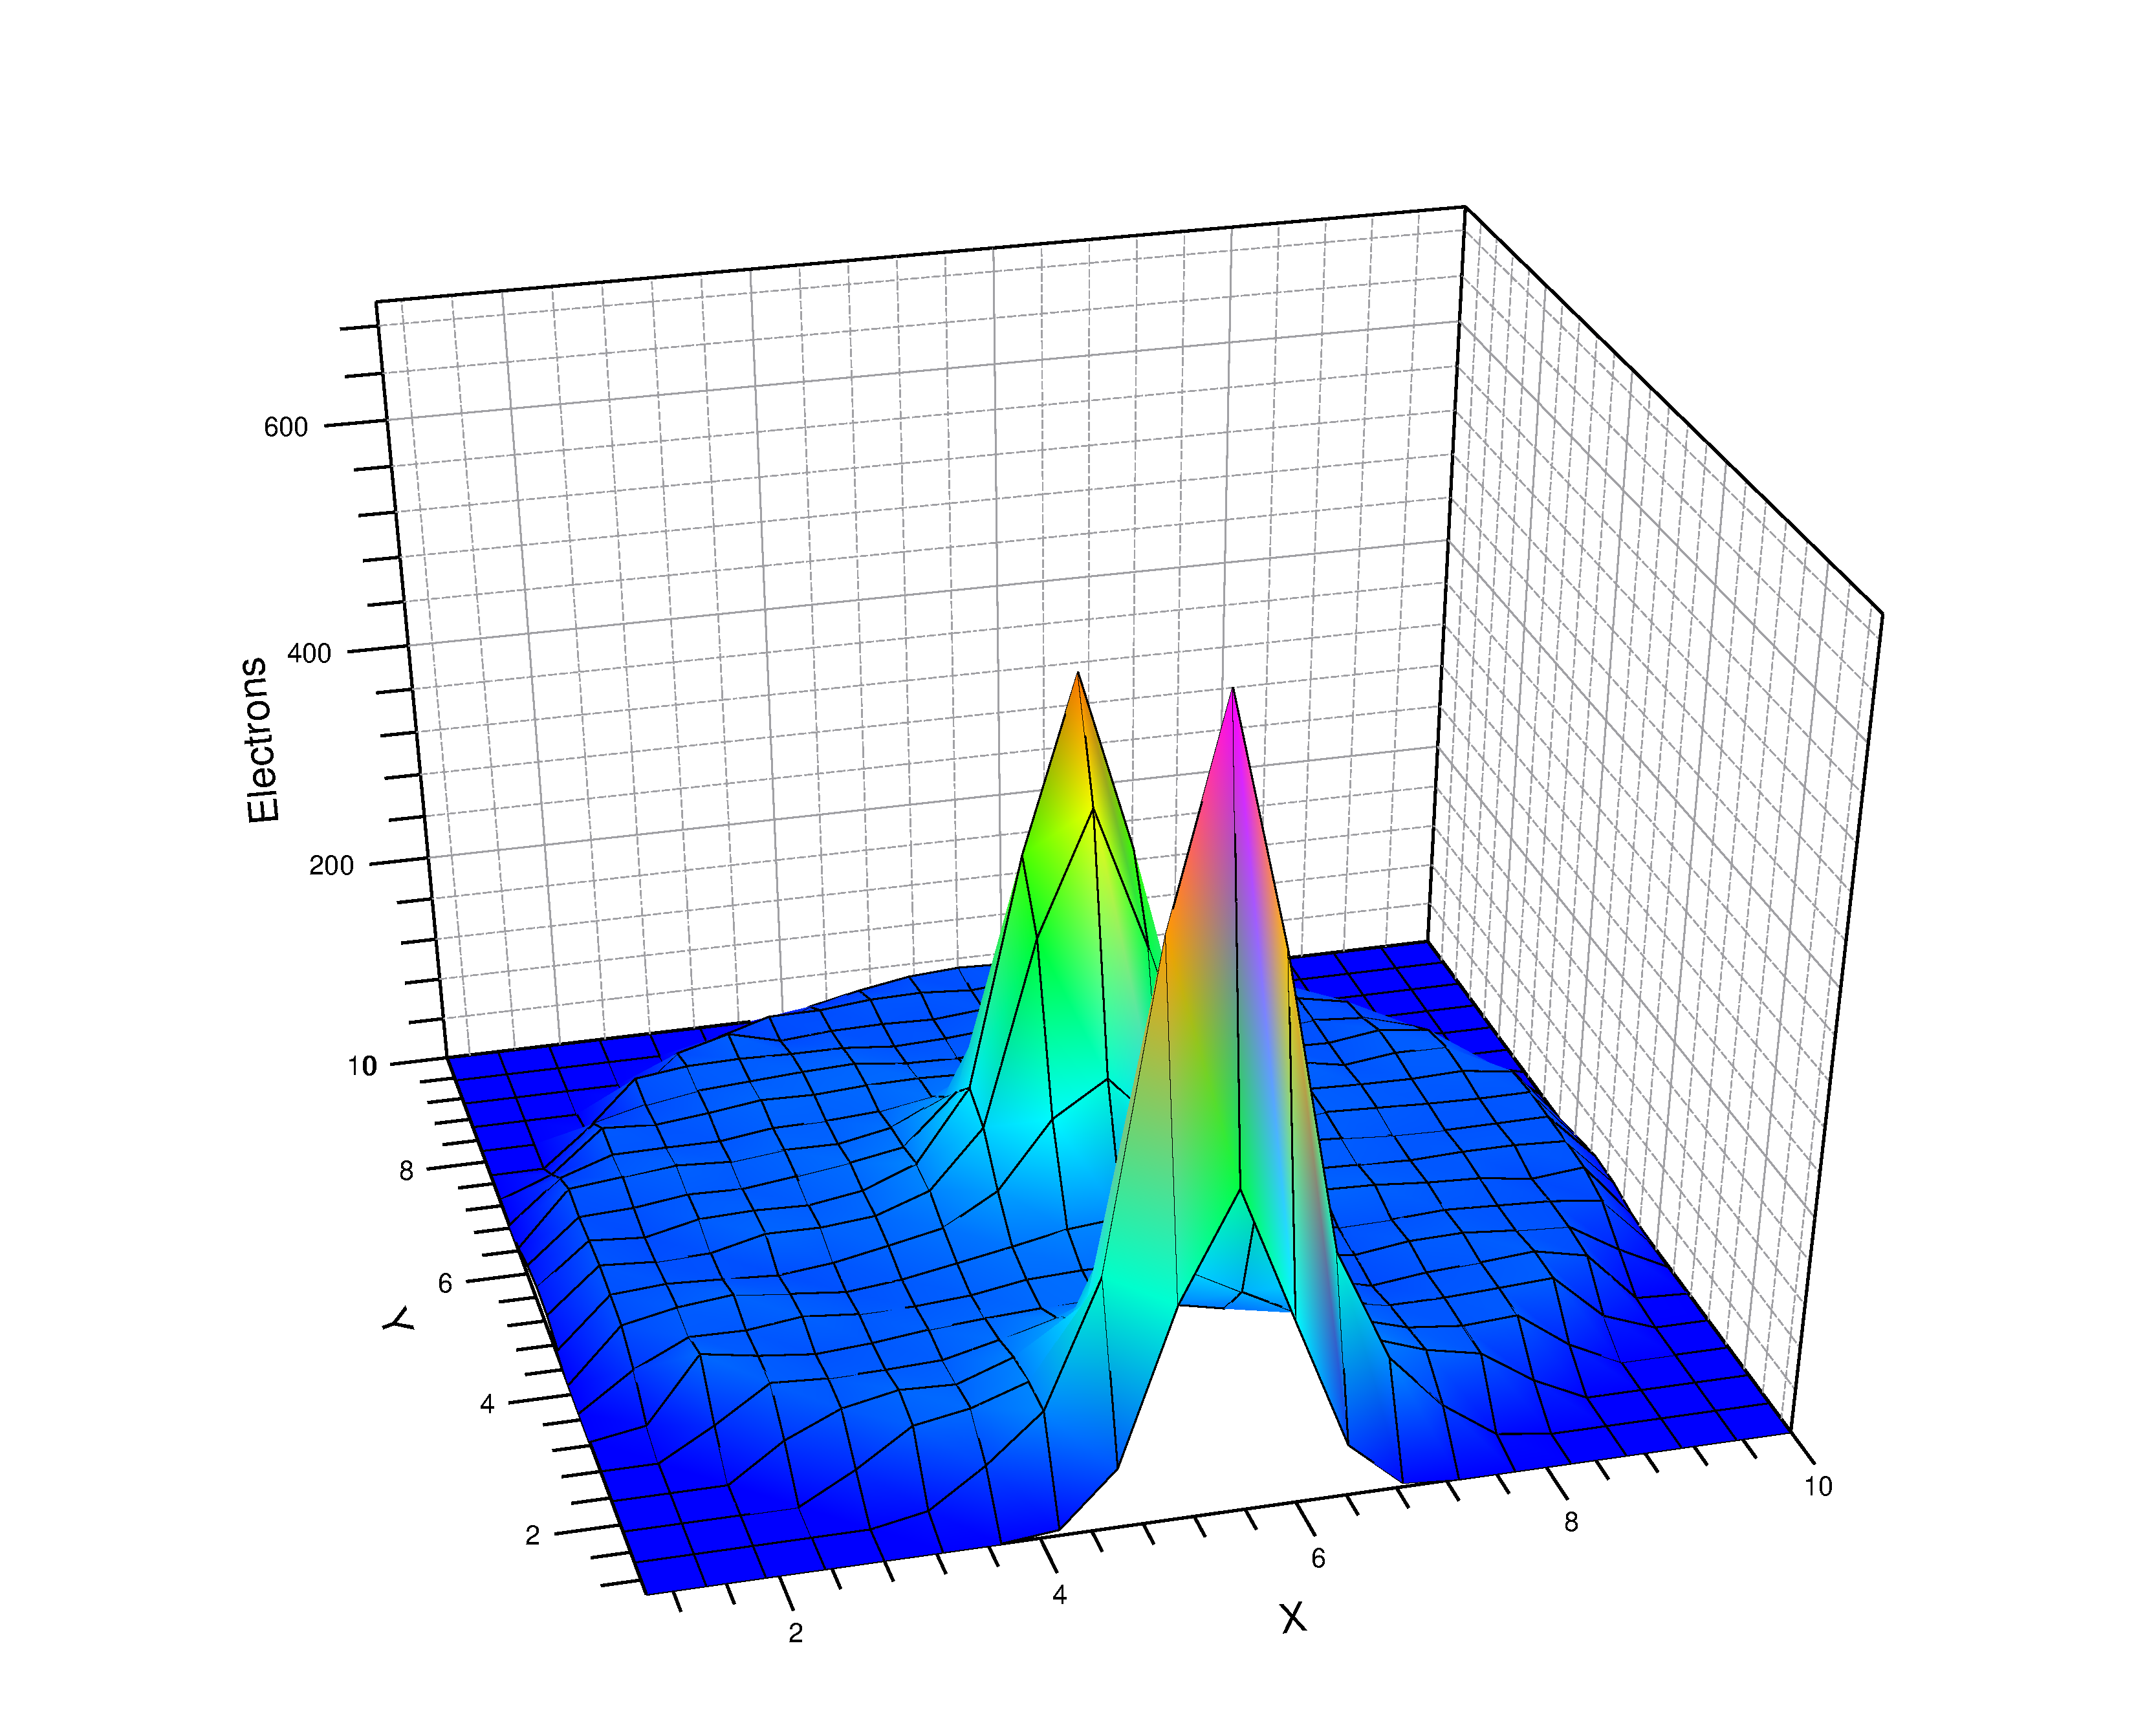
\includegraphics[width=1\textwidth]{fig/etoile divergente red3.pdf}
               \caption{Troisième étoile exclue}
               \label{subfig:exlc3}
           \end{subfigure}
           
      \caption{Photons mesurés par le CCD pour trois étoiles écartées de la calibration (filtre r)}
       \label{fig:exclu}
\end{figure}
\begin{figure}[h]
        \centering
        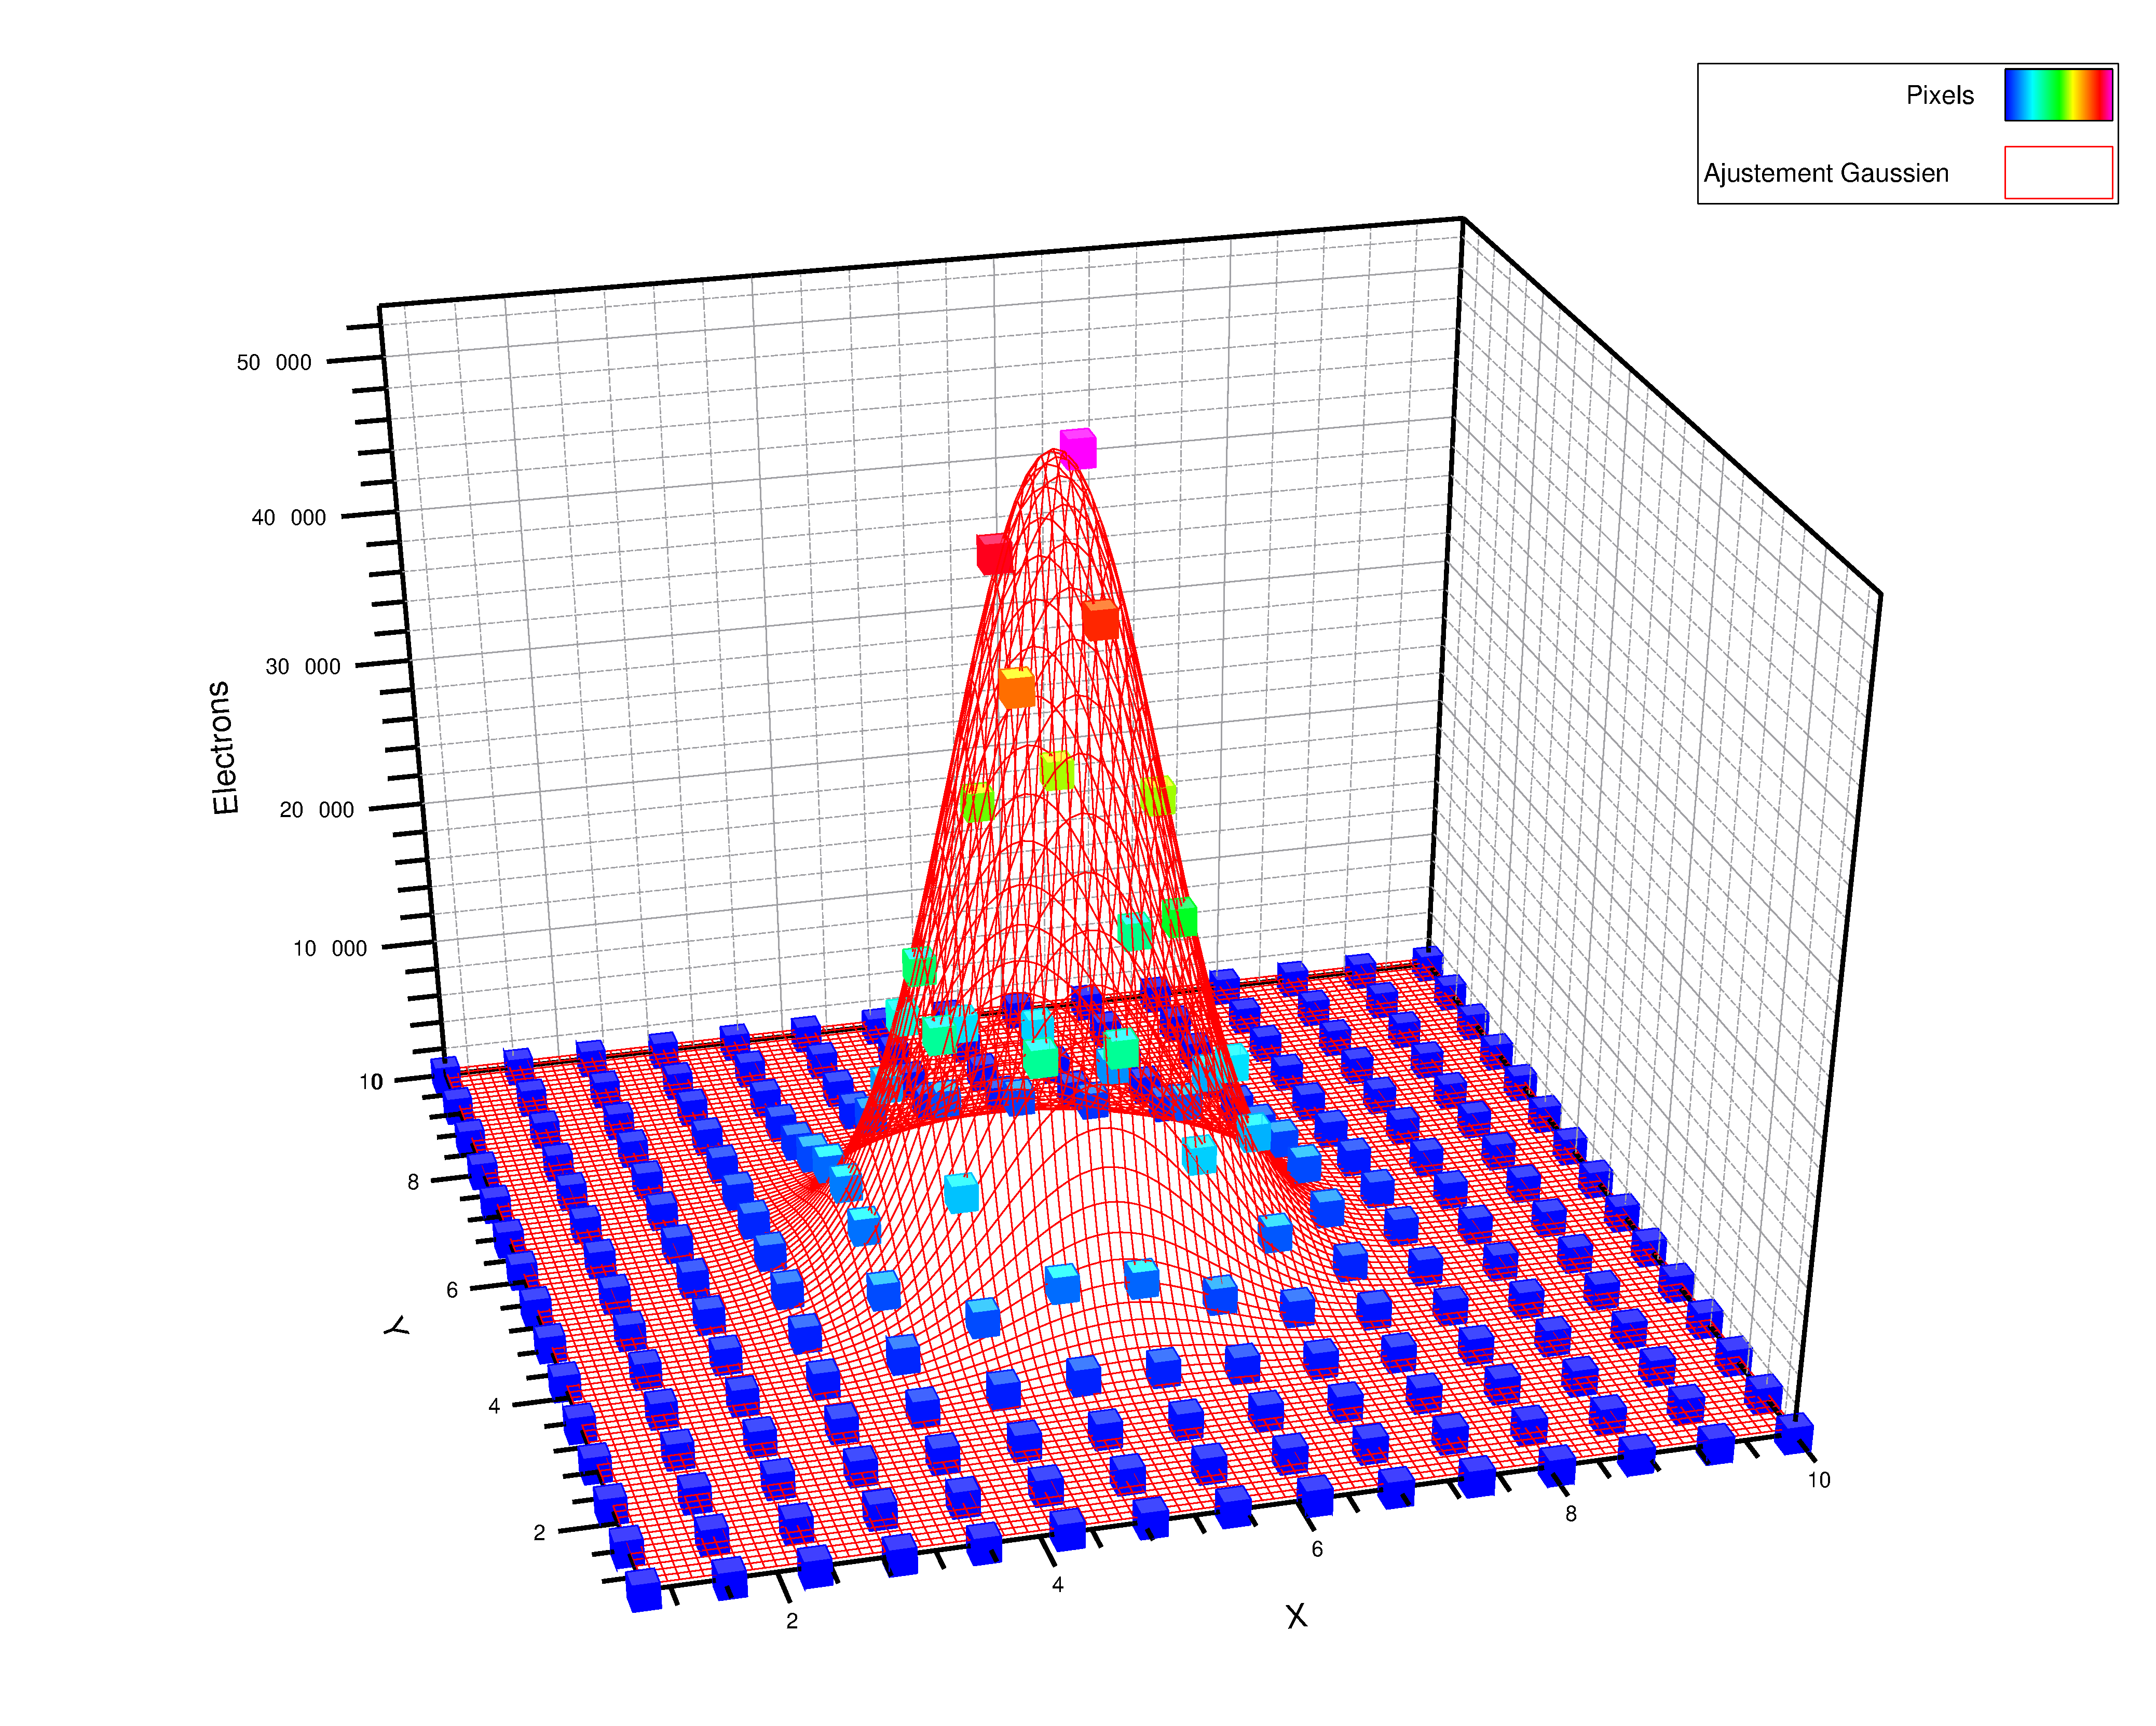
\includegraphics[width=0.7\linewidth]{fig/FWHM.pdf}
        \caption{Visualisation des photons mesurés pour une étoile avec un important rapport signal/bruit\label{fwhm}}
\end{figure}

%
% des annexes peuvent être utilisées pour alléger le texte principal
